Pour ce projet, le robot doit être capable de répondre à trois ordres différents: déplacement en ligne droite et rotation dans les deux sens. Le signal audio qui est envoyé doit donc contenir cet ordre ainsi qu'un paramètre: le nombre (signé) de centimètres à parcourir ou l'angle de rotation en degré. Dans ce chapitre, nous allons développer le chemin que parcourt l'information entre le moment où elle est envoyée sous forme sonore par l'émetteur qui nous a été fourni et la réception par le microcontrôleur.

\section{Codage de l'ordre}
Le message envoyé au robot est codé sur 13 bits. Le premier et le dernier sont des \ilcode{0} et sont respectivement le start bit et le stop bit: ils permettent de détecter le début et la fin d'une trame. Le bit 11 est un bit de parité pour la détection d'erreur. Les \SI{10} bits restant contiennent l'information utile, les deux premiers donnent l'ordre suivant la convention suivante :
\begin{itemize}
\item \ilcode{0b00} : avance tout droit
\item \ilcode{0b01} : tourne à droite
\item \ilcode{0b10} : tourne à gauche
\end{itemize}
Les 8 bits suivants représentent simplement le nombre de degrés ou de centimètres à parcourir.

L'information est modulée en FSK, et le signal audio est généré par un script Matlab ou python fourni. Les paramètres importants pour le dimensionnement de la chaîne d'acquisition et la démodulation sont repris ci-dessous:
\begin{align*}
f_{sym} &= \SI{10}{\hertz} \;(\tau_{sym} = \SI{100}{\milli\second})\\
f_{HI} &= \SI{1100}{\hertz}\\
f_{LO} &= \SI{900}{\hertz}\\
\end{align*}

La chaîne d'acquisition est constituée des différents étages suivants:
\begin{itemize}
\item Le micro
\item L'amplification
\item Le filtre de garde
\item Le convertisseur analogique-numérique
\end{itemize}
Le signal doit être ensuite démodulé à l'aide des éléments suivants:
\begin{itemize}
\item Les filtres passe-bande
\item Les comparateurs
\end{itemize}

Dans les deux section suivantes, nous allons donc passer en revue le dimensionnement de la chaîne d'acquisition et le traitement numérique du signal audio, jusqu'à la sortie du comparateur. Le but final de ce bloc est donc de déterminer, à chaque période d'échantillonnage, si le signal comporte du 900 et/ou du \SI{1100}{\hertz}

\section{Dimensionnement de la chaîne d'acquisition}

\subsection{Le micro}
Notre microphone fournit un signal d'une amplitude maximale de \SI{1}{\milli\volt}. Il doit être polarisé par une résistance de \SI{2.2}{\kilo\ohm} suivant le schéma de la figure \ref{fig:polarisation du micro}.
\begin{figure}[htbp]
\centering
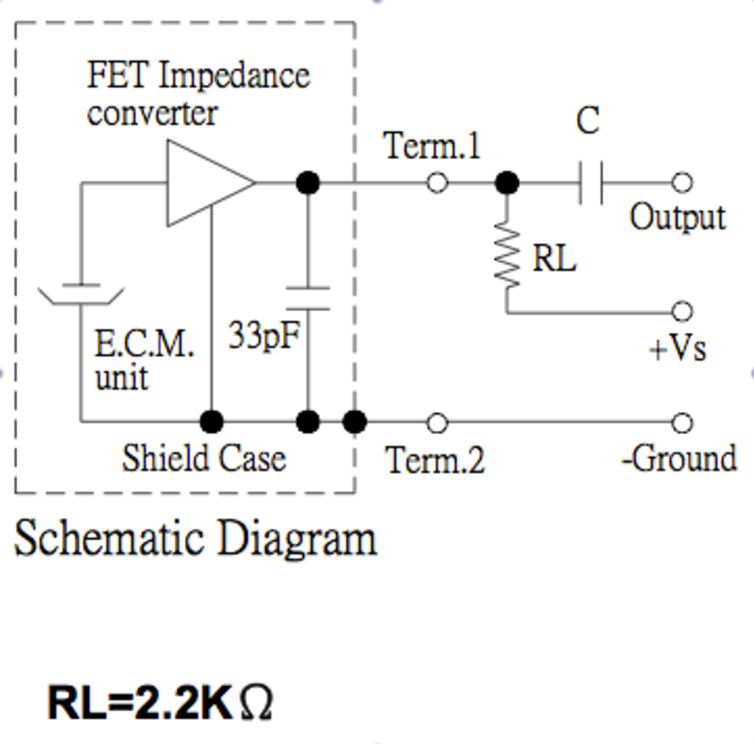
\includegraphics[width=0.7\textwidth]{polarisation_micro.pdf}
\caption{Circuit du microphone}
\label{fig:polarisation du micro}
\end{figure}

Le principe de fonctionnement du micro est que sa membrane extérieure mobile constitue l'armature d'un condensateur chargé en permanence, la deuxième armature étant fixe. Le mouvement de cette membrane, dû aux variations de pression, va modifier la capacité du condensateur, et donc la tension à ses bornes. Le microphone est dit piézoélectrique. Dans notre cas, le microphone est aussi dit "à électret", ce qui signifie qu'il ne nécessite pas d'alimentation pour maintenir le condensateur chargé : le matériau constituant la membrane présente la propriété de conserver une charge électrostatique. Cependant, une alimentation est nécessaire pour polariser le transistor de l'étage de sortie du microphone, au travers de la résistance $R_L$.

\subsection{Montage amplificateur}
Comme nous l'avons dit précédemment, le signal en sortie de notre micro a une amplitude maximale de \SI{1}{\milli\volt}. Le première priorité est donc de l'amplifier afin de préserver le plus possible le SNR pour la suite du traitement.

La plage de tension d'entrée de l'ADC va de \SI{0}{\volt} à \SI{3.3}{\volt}, afin d'occuper cette plage le plus largement possible tout en gardant une marge de sécurité par rapport à la saturation de l'ADC, il est suggéré de dimensionner l'amplification  de façon à centrer le signal sur \SI{1.65}{\volt} et avec une amplitude de \SI{1.5}{\volt}. Pour cela nous avons utilisé deux étages amplificateurs, respectivement d'un gain de 68 et 22. Nous avons donc utilisé le montage représenté à la figure \ref{fig:etage amplificateur}.

Calculons d'abord la tension à la sortie du premier étage ($V_{out 1}$), à l'aide du principe de superposition. On considère d'abord la seule source de tension continue, la capacité est alors un circuit ouvert (\ref{eqn:2.1}):
\begin{figure}[htbp]
\centering
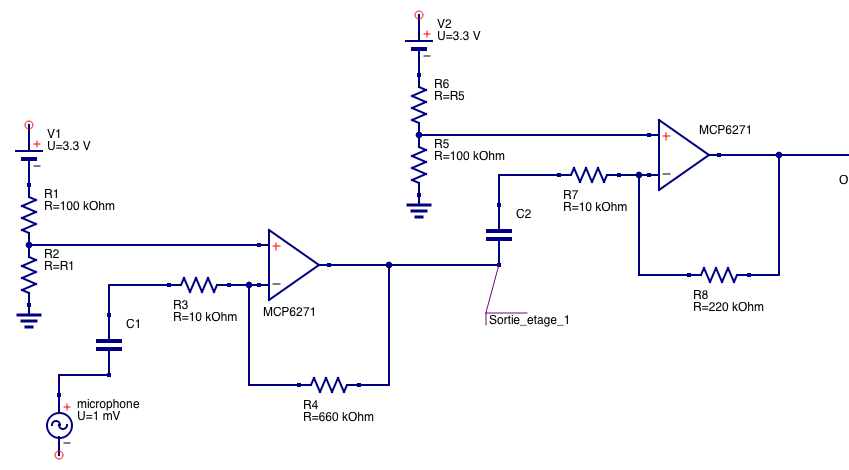
\includegraphics[width=0.7\textwidth]{etage_amplificateur.png}
\caption{Étage amplificateur}
\label{fig:etage amplificateur}
\end{figure}
\begin{equation}
V_{+} = V_{-} = V_{out 1} = \SI{1.65}{\volt}
\label{eqn:2.1}
\end{equation}
Considérons ensuite uniquement la source de tension alternative, le circuit est alors un inverseur classique (\ref{eqn:2.2}) :
\begin{equation}
V_{out 1} = \frac{R_2}{R_1} V_{micro} = 68 V_{in}
\label{eqn:2.2}
\end{equation}
On retrouve la tension en sortie du premier étage en sommant ces deux termes pour finalement obtenir (\ref{eqn:2.3}) :
\begin{equation}
V_{out 1} = \SI{1.65}{\volt} + 68 V_{micro}
\label{eqn:2.3}
\end{equation}

La capacité $C_{2}$ placée entre nos deux étages d'amplification sert à supprimer la composante continue de la tension, la recentrant autour de \SI{0}{\volt}. On évite ainsi de faire saturer notre deuxième ampli-op. Pour le deuxième étage, les calculs sont exactement les mêmes que pour le premier, exception faite du gain du montage inverseur qui vaut 22. On obtient alors notre signal amplifié (\ref{eqn:2.4}) :
\begin{equation}
V_{out final} = \SI{1.65}{\volt} + 1496 V_{micro}
\label{eqn:2.4}
\end{equation}

Pour vérifier le bon fonctionnement de l'étage amplificateur, nous avons effectué des essais sur celui-ci à l'aide du générateur de fonction et du micro. A ce niveau-ci, observer le signal amplifié du micro à l'oscilloscope n'est pas entièrement satisfaisant puisqu'on observe somme toute beaucoup de bruit. Il est cependant possible de vérifier quelques point clés: pas de saturation (plage de sortie du micro conforme à ce qui était attendu), contenu fréquentiel principalement à basse fréquence (FFT ou simplement vérifier le temps caractéristique à l'oscilloscope), et enfin quand même une certaine réaction au son. Les résultats obtenus à l'oscilloscope sont finalement entièrement satisfaisants.

\subsection{Filtre de garde}
\label{Filtre de garde}
Étant donné que nous allons numériser notre signal, il est nécessaire d'utiliser un filtre de garde pour éviter tout repliement spectral. Les spécifications suivantes sont imposées:
\begin{itemize}
\item Filtre Butterworth d'ordre 2
\item L'atténuation maximale des fréquences utiles doit être de 0.99
\item L'atténuation minimale des fréquences filtrées doit être de 0.05.
\end{itemize}
L'amplitude de la réponse en fréquence d'un filtre de Butterworth est donné par l'équation \ref{eqn:butterworth}
\begin{equation}
\vert{H(j\omega)}\vert = \sqrt[]{\frac{1}{1+(\frac{\omega}{\omega_c})^{2n}}}
\label{eqn:butterworth}
\end{equation}
Nous connaissons notre fréquence utile maximale, elle est de \SI{1100}{\hertz}. Si nous injectons cette valeur de $\omega$ dans l'équation, nous pouvons remplacer le terme de gauche par 0.99 et n par 2. On peut alors calculer  l'inconnue restante, $f_c$, qui vaut \SI{2972.97}{\hertz}.

Maintenant que nous connaissons la fréquence de coupure de notre filtre, nous pouvons calculer la fréquence à partir de laquelle il fournira une atténuation d'au moins 20. On remplace dans l'équation \ref{eqn:butterworth} le module de la réponse en fréquence par 0.05, n par 2 et $f_c$ par \SI{2972.97}{\hertz}. On obtient comme valeur de $f_{\SI{-26}{\deci\bel}}$ \SI{13.287}{\kilo\hertz}.

Avec toutes ces informations, nous avons utilisé l'outil "Filter Wizard" d'Analog Devices \footnote{\url{http://www.analog.com/designtools/en/filterwizard}} qui nous a permis de designer notre filtre.
\begin{figure}[htbp]
\centering
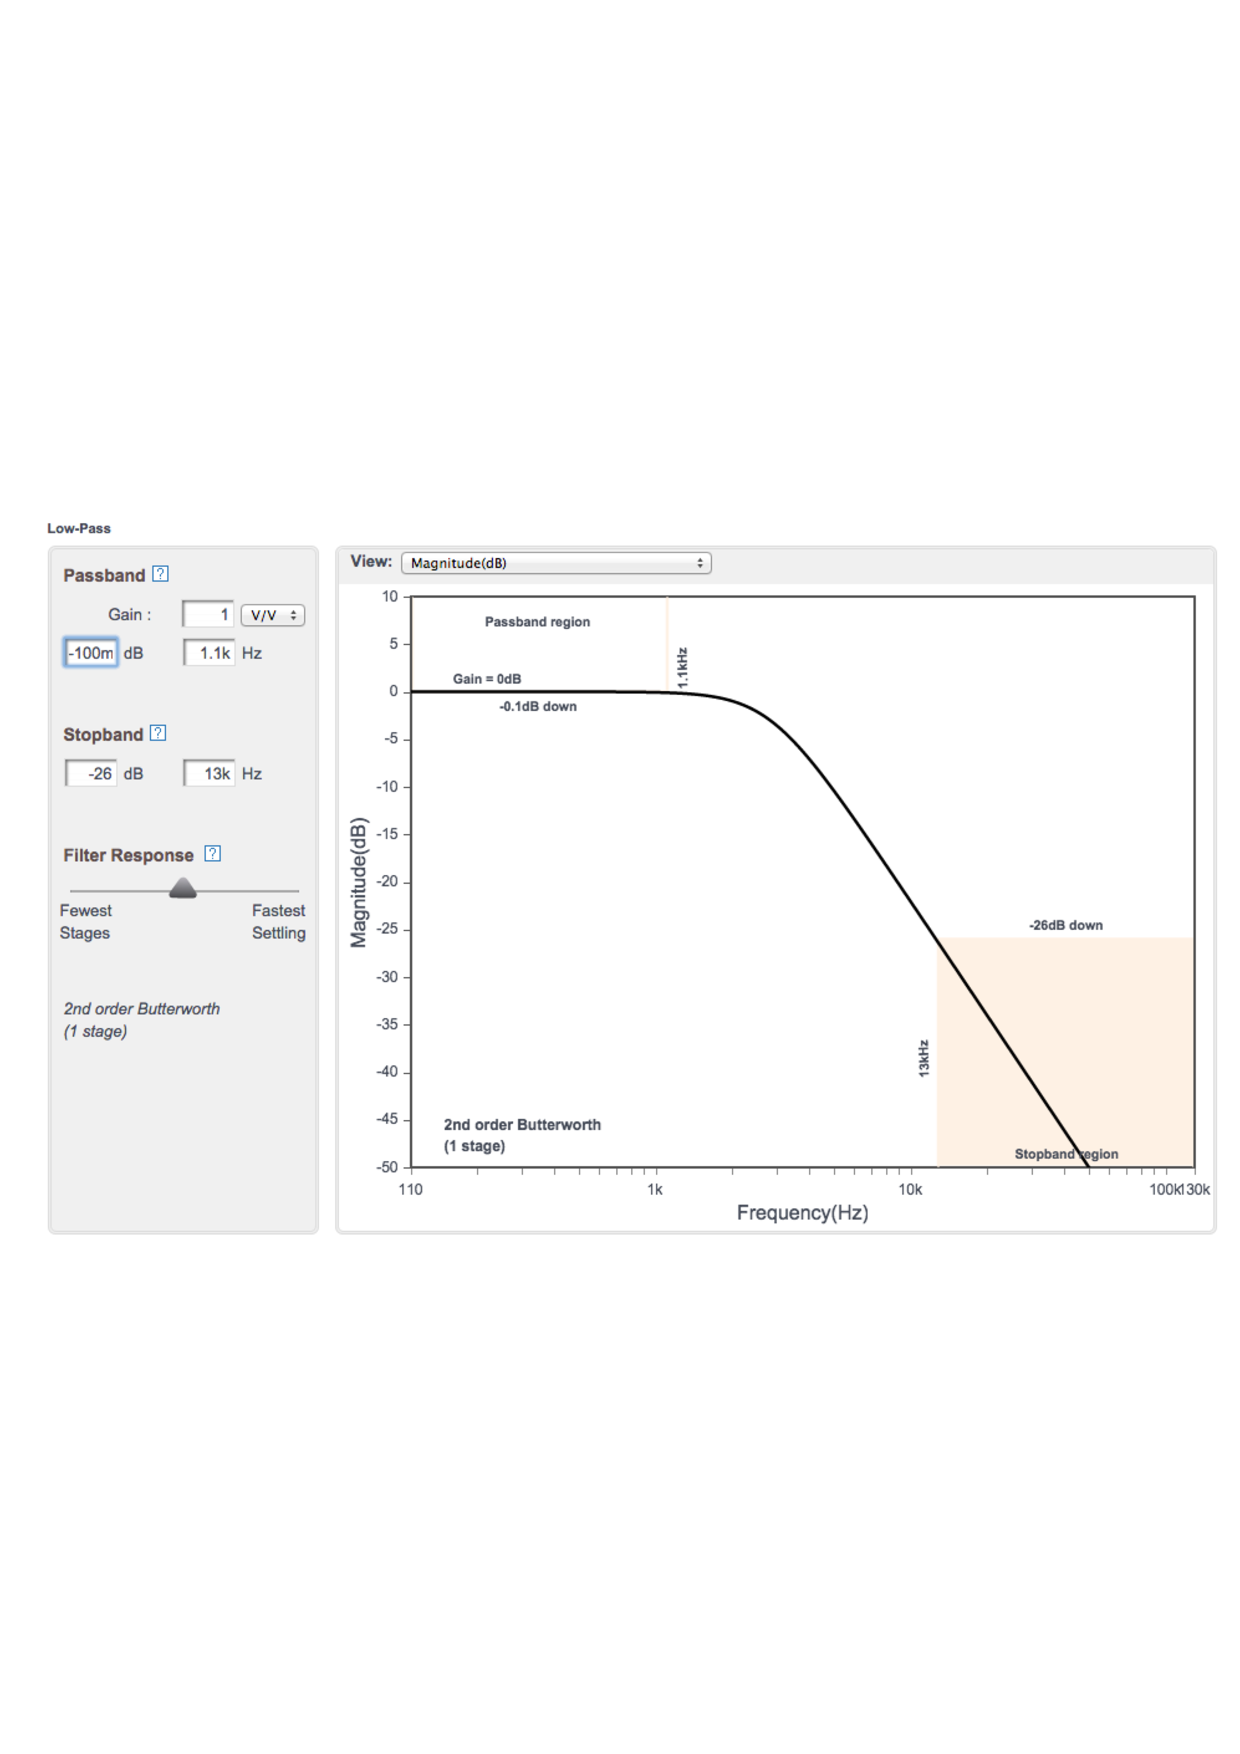
\includegraphics[width=\textwidth]{specs_filtre_analog.pdf}
\caption{L'interface du "Filter Wizard"}
\label{fig:specsAnalogFilter}
\end{figure}
La figure \ref{fig:specsAnalogFilter} montre les spécifications de notre filtre analogique ainsi que l'amplitude de sa réponse en fréquence en fonction de la fréquence. Pour l'implémentation du filtre, Analog nous conseillait un étage Sallen-Key, ce que nous avons fait.
\begin{figure}[htbp]
\centering
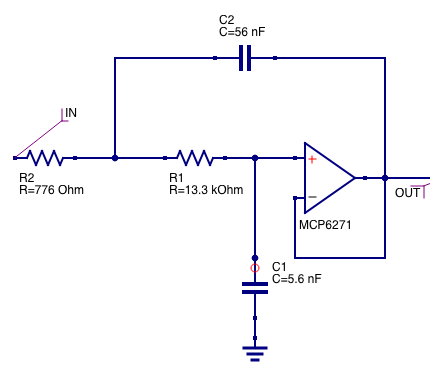
\includegraphics[width = 0.7\textwidth]{filtre_analogique.png}
\caption{Montage de notre filtre analogique}
\label{fig:filtreAnalogique}
\end{figure}
La figure \ref{fig:filtreAnalogique} montre le montage de notre filtre passe-bas. Pour tester notre implémentation, nous lui avons mis en entrée des sinus à différentes fréquences\footnote{Nous avons d'abord essayé de faire une FFT de la réponse impulsionnelle à l'aide de générateur de PWM et de l'oscilloscope, mais cela n'a pas été concluant car la résolution fréquentielle de l'oscilloscope est trop mauvaise et aussi probablement parce que le pulse le plus étroit que peut fournir le générateur est encore trop large.}: \SI{900}{\hertz}, \SI{1100}{\hertz}, \SI{13}{\kilo\hertz} (première fréquence atténuée avec un facteur 0.05) et à la fréquence de coupure (\SI{2972.97}{\hertz}). Les résultats sont exposés aux figures \ref{fig:filtreAnalog900Hz}, \ref{fig:filtreAnalog1100Hz}, \ref{fig:filtreAnalog13kHz} et \ref{fig:filtreAnalogFc}. L'entrée est représentée en rouge et la sortie en bleu.
\begin{figure}[htbp]
\centering
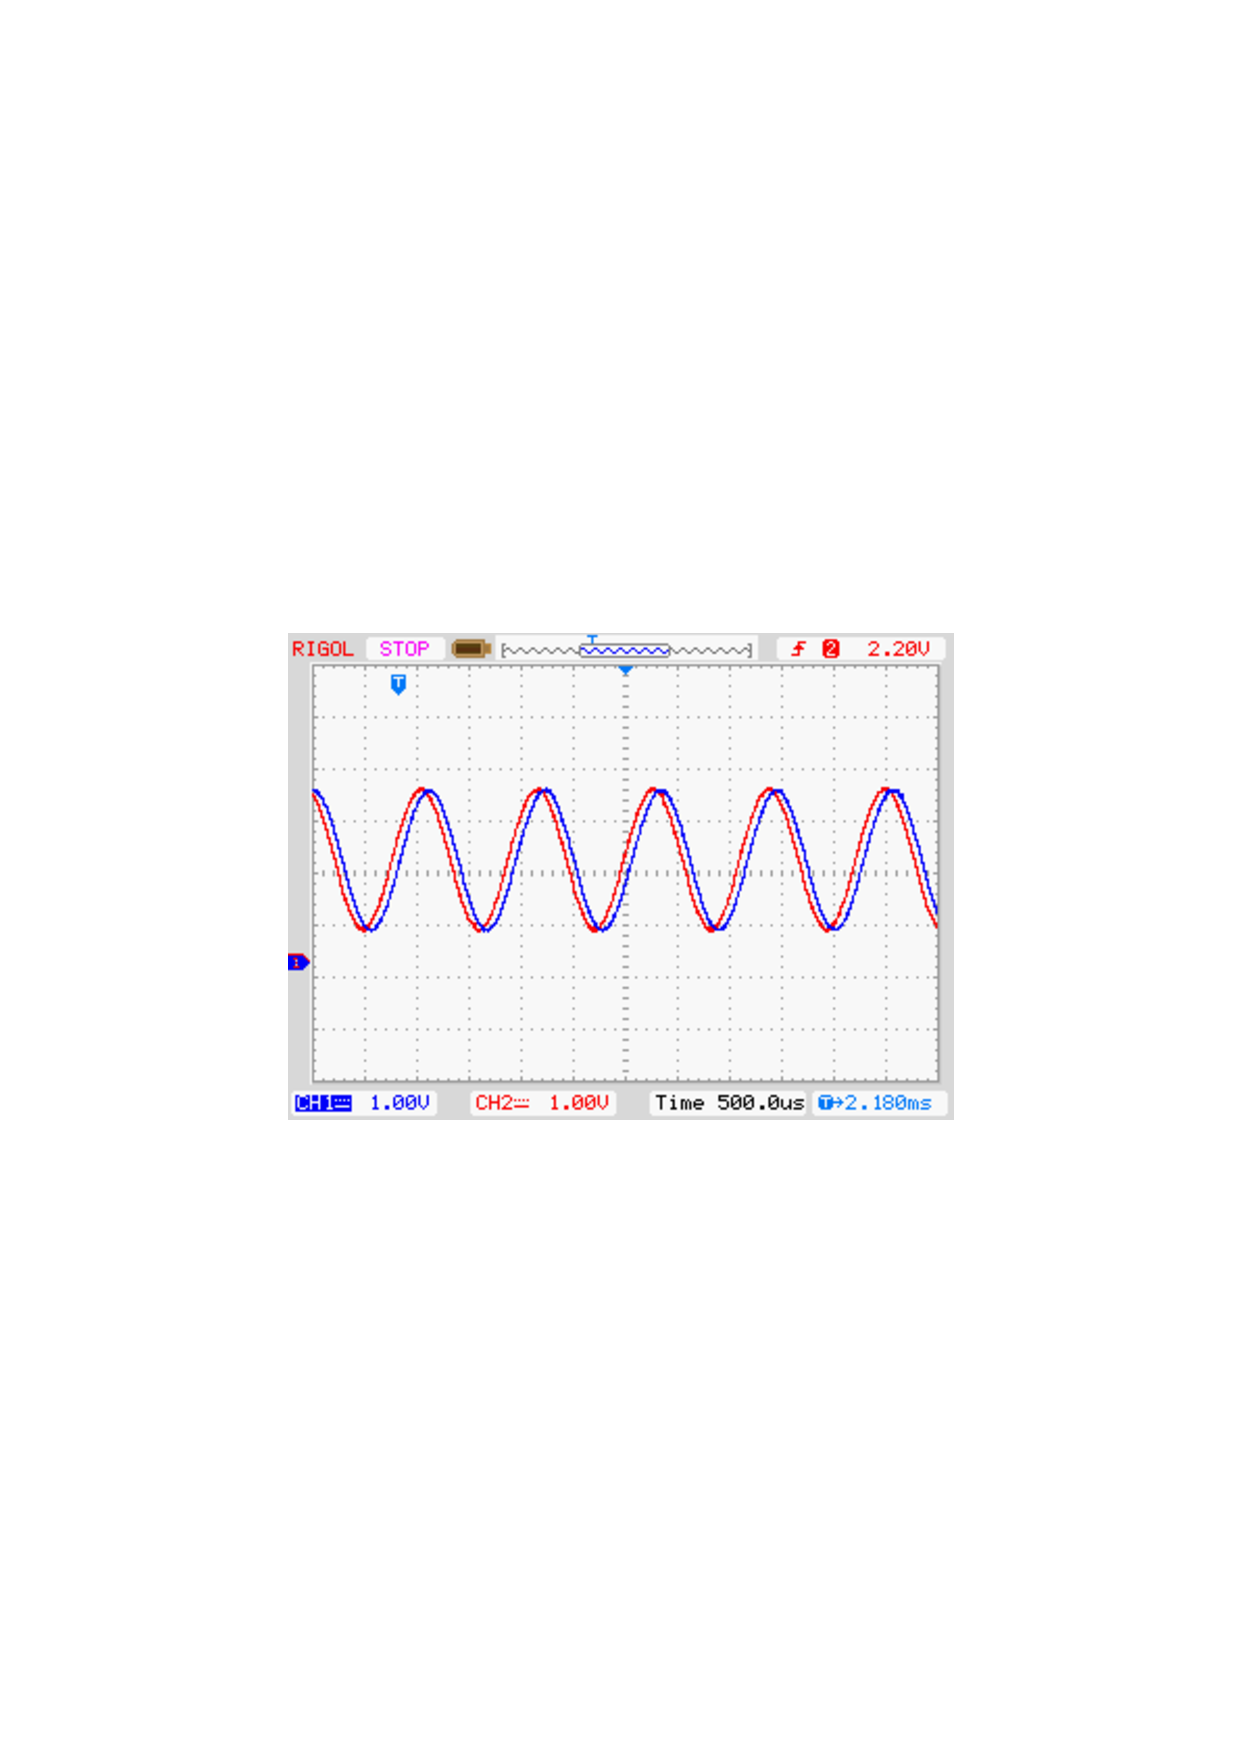
\includegraphics[width = 0.7\textwidth]{filtreAnalog900Hz.pdf}
\caption{Sortie (bleu) du filtre de garde pour une entrée à \SI{900}{\hertz} (rouge)}
\label{fig:filtreAnalog900Hz}
\end{figure}
\begin{figure}[htbp]
\centering
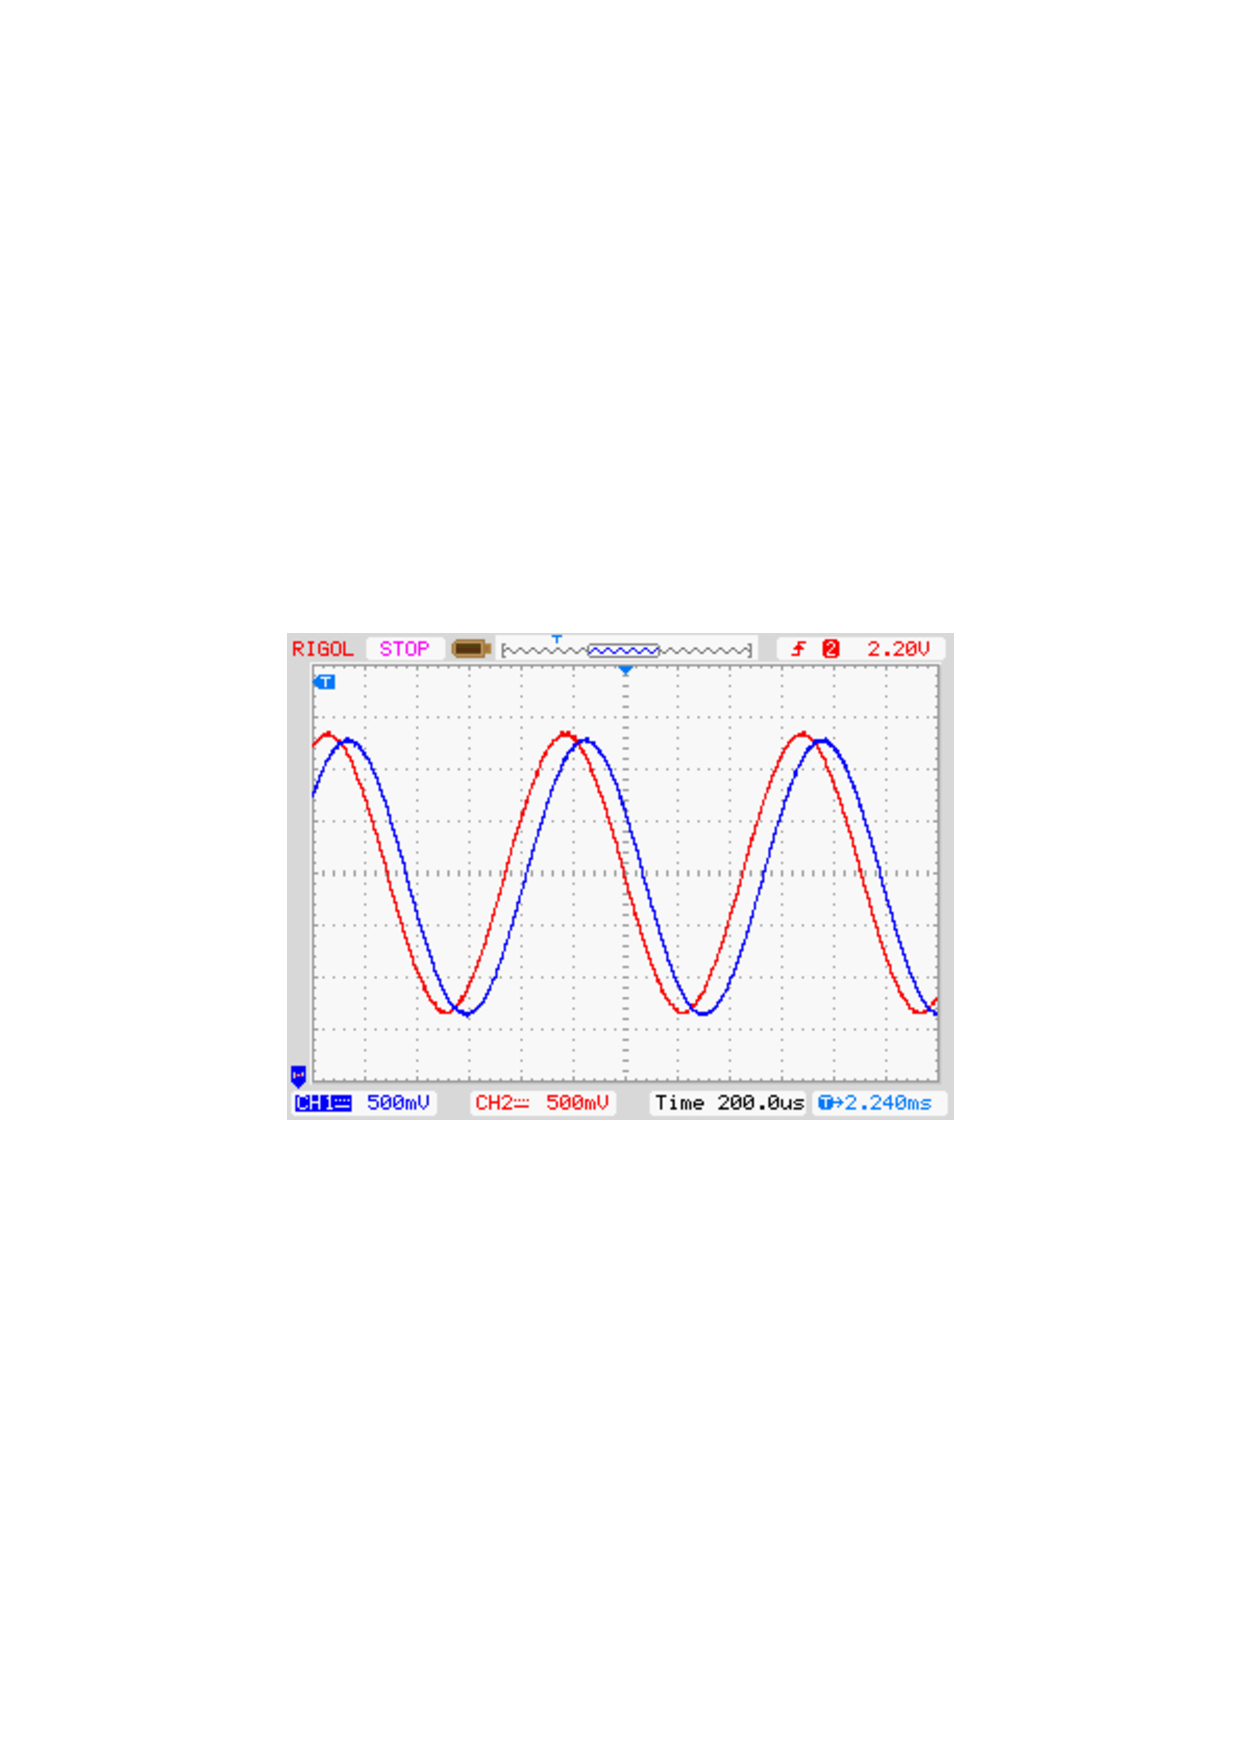
\includegraphics[width = 0.7\textwidth]{filtreAnalog1100Hz.pdf}
\caption{Sortie (bleu) du filtre de garde pour une entrée à \SI{1100}{\hertz} (rouge)}
\label{fig:filtreAnalog1100Hz}
\end{figure}
\begin{figure}[htbp]
\centering
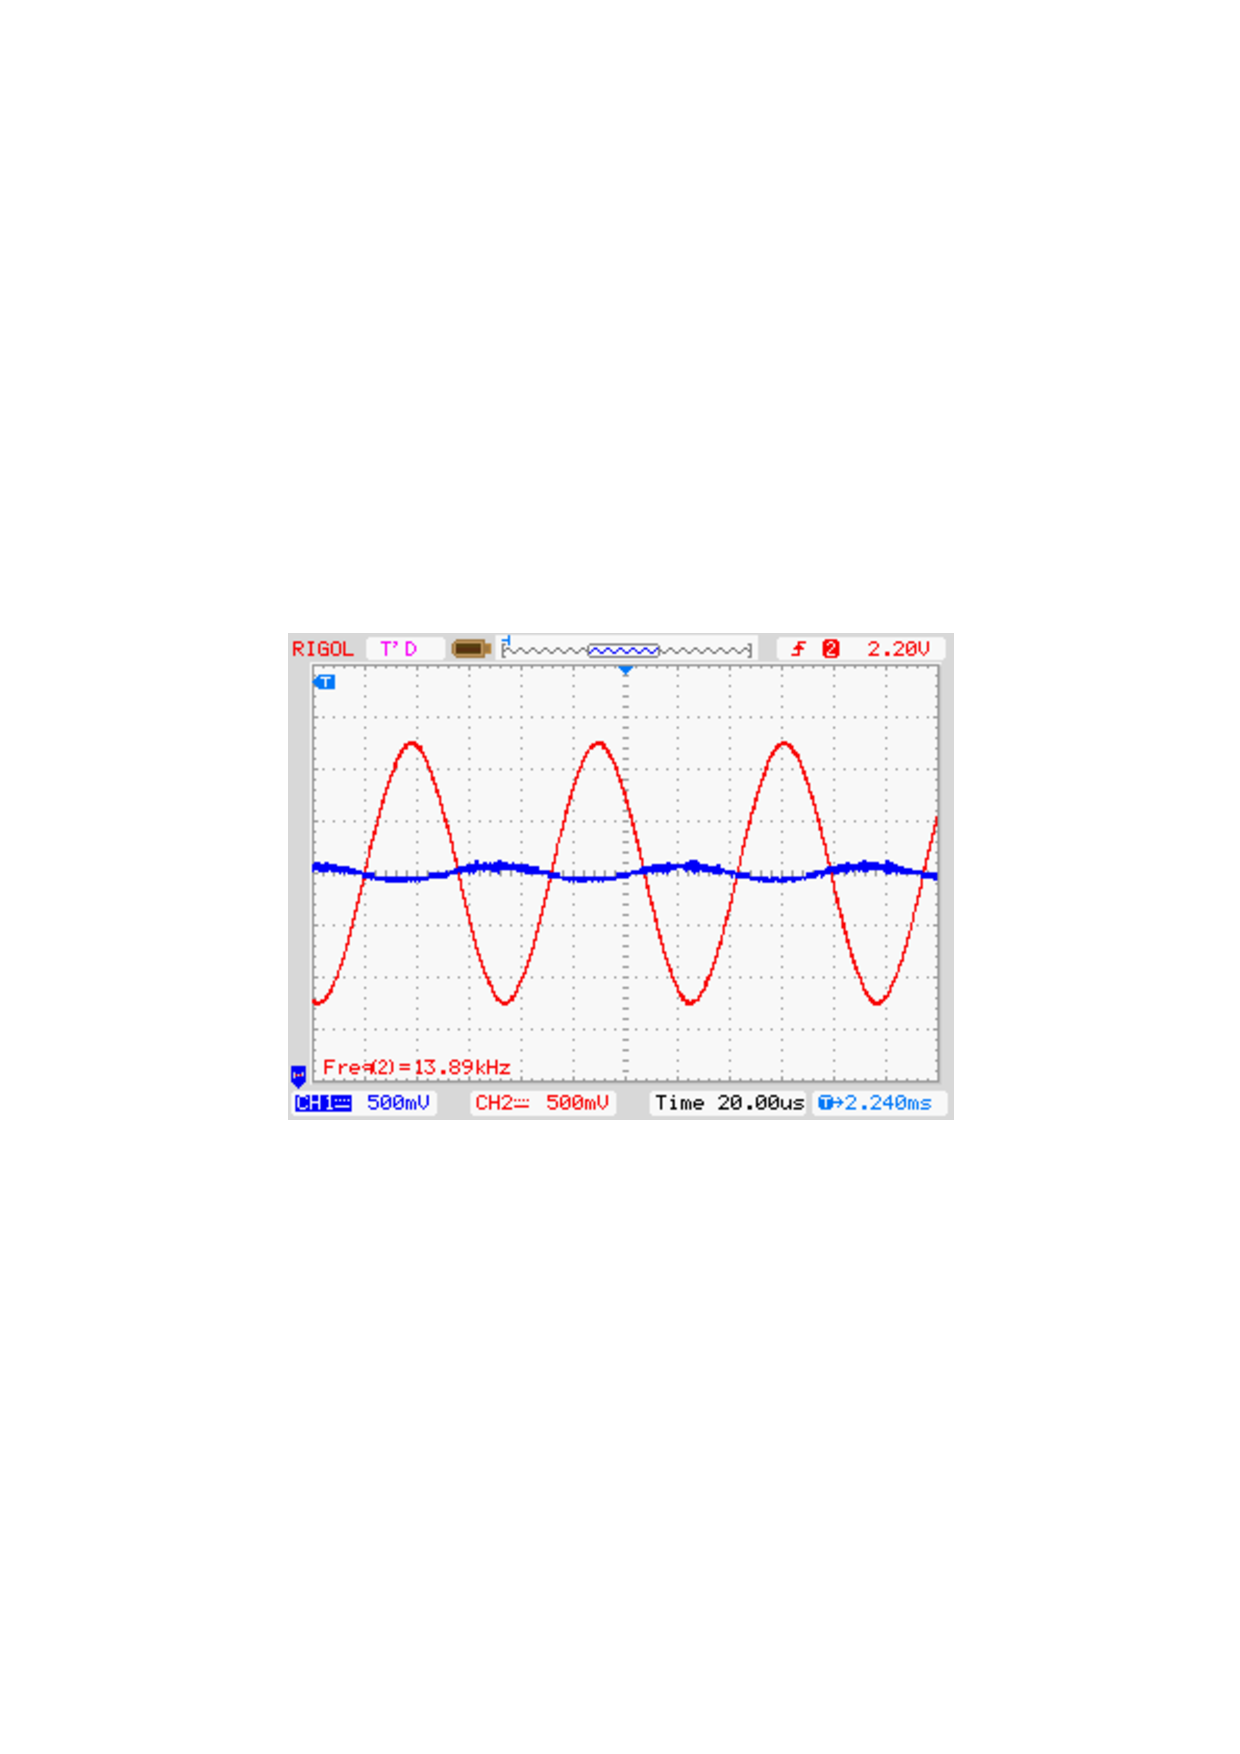
\includegraphics[width = 0.7\textwidth]{filtreAnalog13kHz.pdf}
\caption{Sortie (bleu) du filtre de garde pour une entrée à \SI{13}{\kilo\hertz} (rouge)}
\label{fig:filtreAnalog13kHz}
\end{figure}
\begin{figure}[htbp]
\centering
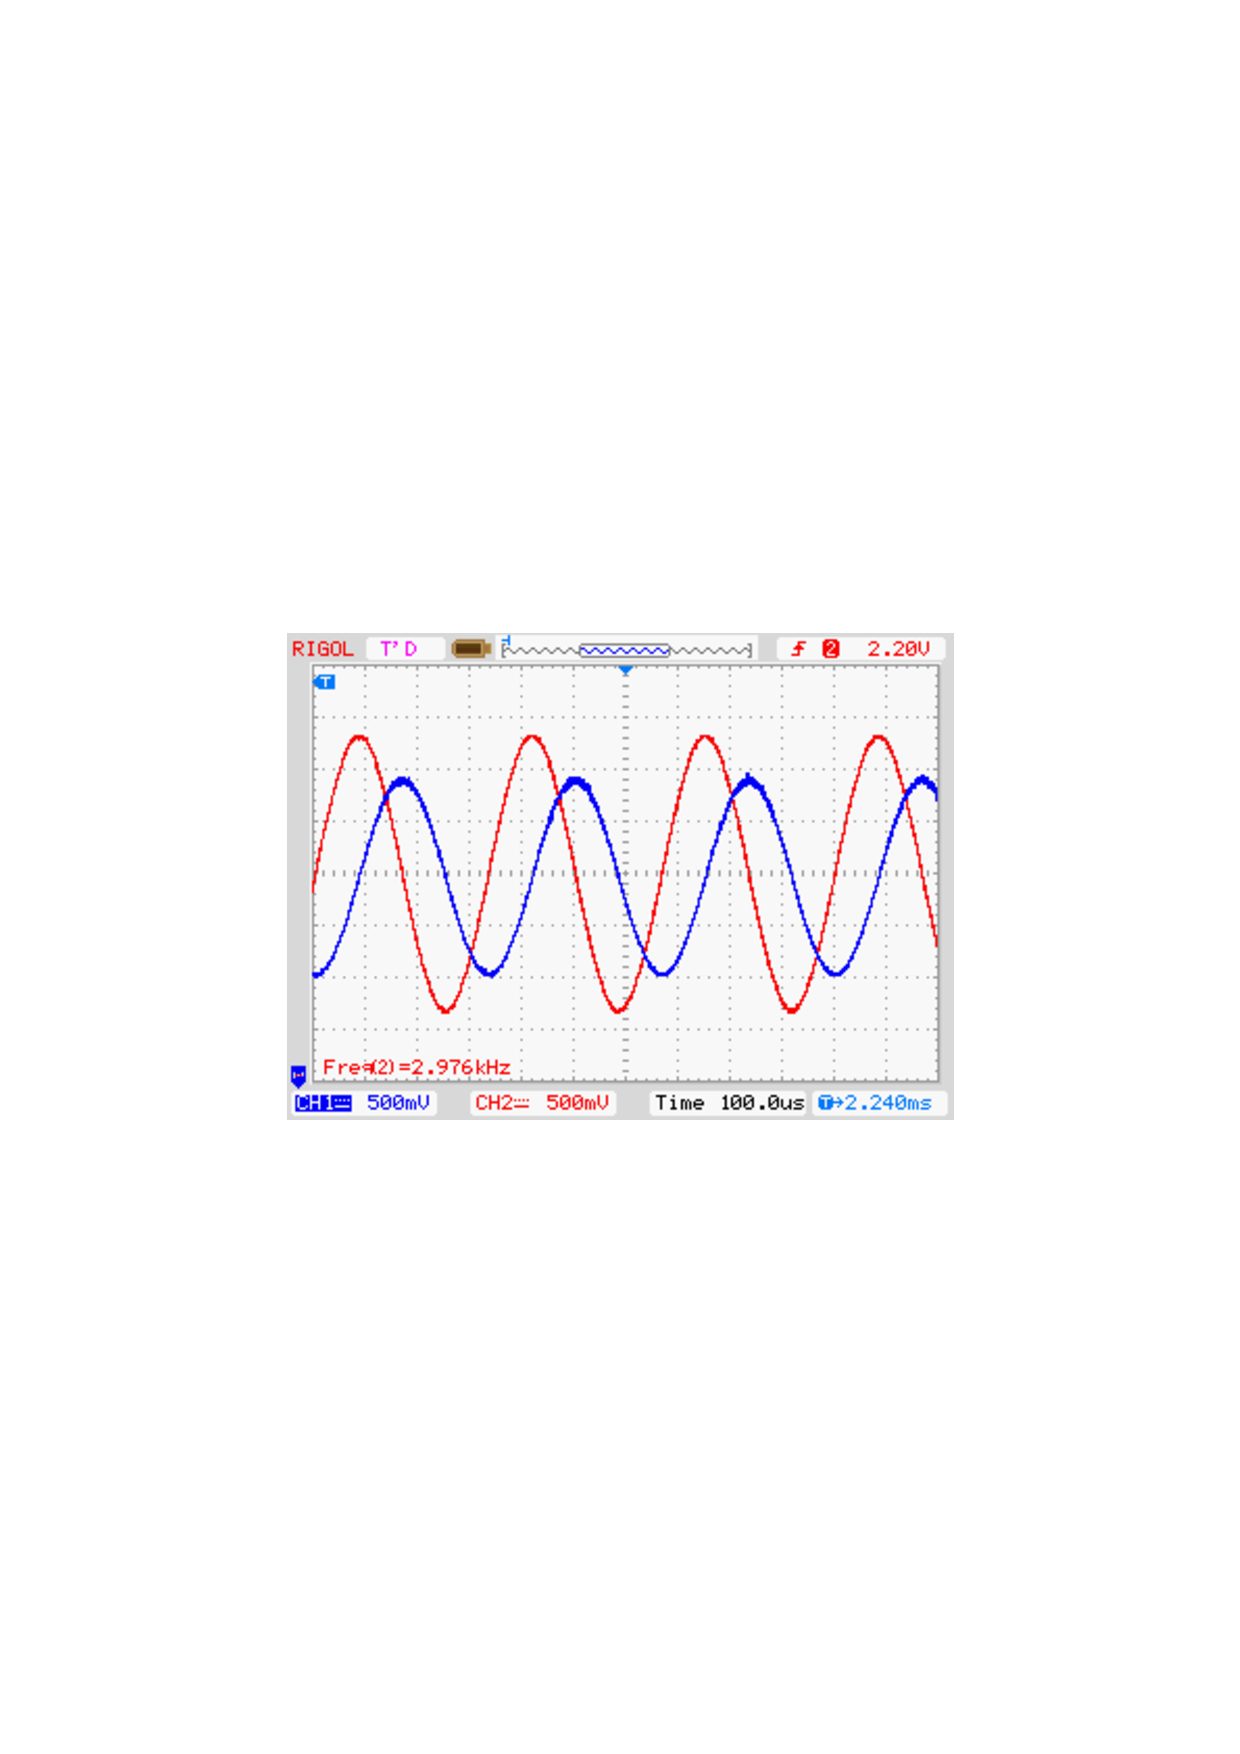
\includegraphics[width = 0.7\textwidth]{filtreAnalogFc.pdf}
\caption{Sortie (bleu) du filtre de garde pour une entrée à la fréquence de coupure (rouge)}
\label{fig:filtreAnalogFc}
\end{figure}

\subsection{Convertisseur analogique-numérique}
Afin que notre microcontrôleur chargé de la communication puisse interpréter les consignes qui lui sont envoyées, il a bien sûr fallu convertir le signal reçu en signal numérique. Pour cela nous avons configuré l'ADC du microcontrôleur communication : c'est la fonction \ilcode{initADC()} qui contient le code correspondant. Ci-dessous nous listons quelques éléments importants de cette configuration :
\begin{itemize}
\item L'ADC fonctionne en mode 12 bits, ce qui est son maximum
\item La tension de référence pour la conversion est la même que la tension d'alimentation
\item L'ADC commence automatiquement à échantillonner lorsqu'il termine une conversion
\item L'ADC déclenche une conversion à chaque période du timer 3, dont la période est \SI{50}{\micro\second} ($f_s = \SI{20}{\kilo\hertz}$)
\item Chaque conversion entraîne une interruption
\end{itemize}
Ce dernier point est particulièrement important, car c'est dans cette interruption que se déroule en fait tout le traitement numérique du signal audio. La trame sortant de l'ADC y est filtrée par deux filtres numériques, et les sorties passent ensuite chacune dans un détecteur de crête. Ceci fait office de démodulation; la trame est ensuite reconstituée par la fonction \ilcode{fskDetector}, qui est déjà fournie. Tout ceci est couvert dans la section suivante, après que la chaîne d'acquisition a été validée.

\subsection{Validation de la chaîne d'acquisition}

Pour valider la chaîne d'acquisition dans son ensemble, un signal audio est généré à une fréquence connue, dans des conditions réelles\footnote{Source audio éloignée de \SIrange{20}{30}{\centi\meter}, test dans le laboratoire qui est raisonnablement bruité.}, et les 100 derniers échantillons sont gardés dans un array qui est ensuite exporté grâce au mode debug et représenté. Ces tests ont été effectués pour 900, 1100, 3000 ($f_c$) et 18900 (première fréquence repliée dans le signal utile) \si{\hertz} et ont tous été concluants (signal suffisamment préservé ou atténué).

\section{Traitement numérique du signal}
Une fois notre signal numérisé, il faut encore en extraire la commande, s'il y en a bien une. Pour cela nous devons détecter la présence de nos deux fréquences de modulation : \SI{900}{\hertz} et \SI{1100}{\hertz}. En pratique, on filtre le signal de façon à ce que toutes les autres fréquences soient atténuées et on vient ensuite vérifier si l'amplitude du signal dépasse encore un certain seuil. Ces deux tâches incombent respectivement aux fonctions \ilcode{filterNewSample(unsigned int sample, int returnArray[2])} et \ilcode{peakDetect(int input[2])}.

\subsection{Filtres numériques passe-bande}
Les filtres sont des filtres récursifs du second ordre. Ils sont décrits par l'équation récursive \ref{eqn:filtre_recursif} que l'on retrouve dans la fonction \ilcode{recurrence(long a1, long a2, long gain,int arrayX[3], long arrayY[3])} ou par le schéma bloc de la figure \ref{fig:filtre_bloc}.
\begin{equation}
y(n) = b_0x(n) + b_1x(n-1) + b_2x(n-2) - a_1y(n-1) - a_2y(n-2)
\label{eqn:filtre_recursif}
\end{equation}
\begin{figure}[htbp]
\centering
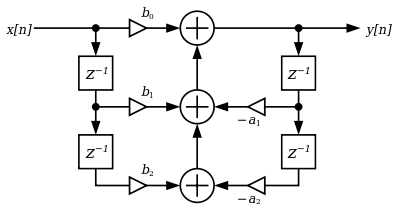
\includegraphics[width=0.7\textwidth]{filtre_bloc.png}
\caption{Schéma bloc d'un filtre numérique du second ordre}
\label{fig:filtre_bloc}
\end{figure}

Nous avons utilisé l'outil \ilcode{fdatool} de Matlab pour trouver les coefficients de nos deux filtres. En donnant comme paramètres au programme les spécifications qui nous étaient imposées, les filtres obtenus étaient composés de quatre sections d'ordre 2. Nous avons commencé par tester ces filtres de manière indépendante du reste du montage et ils fonctionnaient alors très bien. Cependant quand on les plaçait derrière notre ADC, les sorties des filtres n'avaient plus aucun sens. Après un moment, nous nous sommes aperçu que nos filtres étaient tout simplement trop lents: le temps de calcul nécessaire ralentissait le fonctionnement de l'ADC (nous rappelons que le filtrage a lieu dans l'interruption de l'ADC). Pour nous en rendre compte, nous avons flippé un bit sur une des pattes du microcontrôleur dans cette même interruption de l'ADC et nous avons mesuré la fréquence du signal ainsi obtenu à l'oscilloscope. Si l'ADC arrive à fonctionner à la fréquence d'échantillonnage $f_s$  prévue, la fréquence mesurée doit être égale à $\frac{f_s}{2}$ (le bit est flippé à chaque interruption de l'ADC, une période représente donc deux périodes de l'ADC). Nous avons donc tenté de rendre nos filtres plus rapides en modifiant le code, notamment en remplaçant tous les nombres de type \ilcode{float} par des \ilcode{int}, mais aussi en utilisant la connaissance de certains coefficients toujours nuls ou unitaires. Les courbes de Bode du filtre à une seule section centré autour de \SI{900}{\hertz} que nous utilisons pour finir sont données à la figure \ref{fig:filtre_1section}.
\begin{figure}[htbp]
\centering
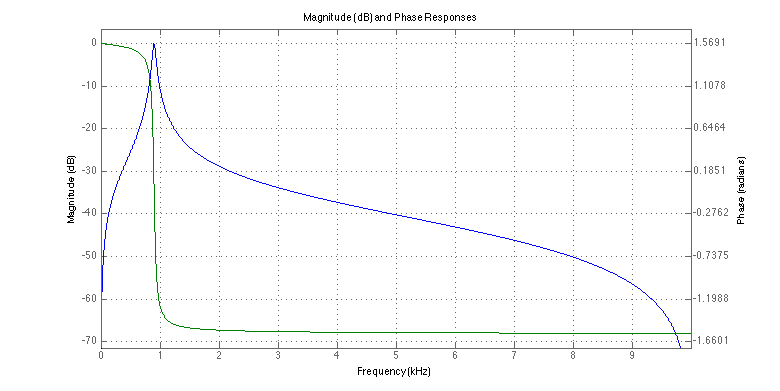
\includegraphics[width=\textwidth]{filtre_1section.png}
\caption{Courbes de Bode du filtre numérique centré autour de \SI{900}{\hertz}}
\label{fig:filtre_1section}
\end{figure}

\subsection{Détecteurs de crête}
Derrière les filtres numériques, le signal passe dans deux comparateurs chargés de détecter la présence de \SI{900}{\hertz} ou \SI{1100}{\hertz}. Pour cela, le microcontrôleur garde en mémoire un bloc du signal correspondant à une période de \SI{1/900}{\second} ou \SI{1/1100}{\second} et trouve le maximum sur ce bloc. Si ce maximum dépasse un certain seuil, la fréquence correspondante est considérée présente. Ces informations sont alors transmises à la fonction \ilcode{fskDetector(int detLow, int detHigh)} qui va mettre en forme la trame détectée.

\subsection{Validation du bloc <<communication audio>>}
Chronologiquement, ce bloc a été achevé en dernier, son fonctionnement a donc été prouvé par le fonctionnement du robot dans son ensemble et sa réponse aux ordre reçus. On observe cependant que la portée de la communication est extrêmement limitée (\SIrange{30}{40}{\centi\meter} maximum dans la direction la plus favorable), et dépend fortement de la direction\footnote{Cela est aussi dû à la forte directionnalité des enceintes de portable utilisées}.